\section{Sistemas dinámicos}

\subsection{Teoría cualitativa}

La teoría cualitativa de las ecuaciones diferenciales se remonta a H. Poincaré y A. M. Lyapunov (estabilidad del movimiento). Empezamos por el sistema lineal plano
\[
    (S) \quad
    \begin{cases}
        u' = a u + b v \\
        v' = c u + d v
    \end{cases}
    \qquad a, b, c, d \in \mathbb{R},
    \qquad \text{es decir,} \quad
    \begin{pmatrix} u \\ v \end{pmatrix}' = \underbrace{\begin{pmatrix} a & b \\ c & d \end{pmatrix}}_{A} \begin{pmatrix} u \\ v \end{pmatrix}.
\]
Estudiar la \textbf{dinámica} de $(S)$ (y, más adelante, de $u' = f(u, v)$, $v' = g(u, v)$) significa representar las trayectorias de todas sus soluciones:
\[
    \Gamma_{(u_0, v_0)} = \{ (u(t), v(t)) : t \in J, \ (u(0), v(0)) = (u_0, v_0) \}.
\]

\subsubsection{Caso 1: autovalores reales y distintos}

Sea $\sigma(A) = \{ \lambda, \mu \}$ con $\lambda \neq \mu$, $\lambda, \mu \in \mathbb{R}$, y sean
\[
    N[A - \lambda I] = L\left[ \begin{pmatrix} \alpha \\ \beta \end{pmatrix} \right], \qquad
    N[A - \mu I] = L\left[ \begin{pmatrix} \gamma \\ \delta \end{pmatrix} \right], \qquad
    P = \begin{pmatrix} \alpha & \gamma \\ \beta & \delta \end{pmatrix}.
\]
Como las columnas de $P$ son autovectores,
\[
    A P = \left( A \begin{pmatrix} \alpha \\ \beta \end{pmatrix} \Bigm| A \begin{pmatrix} \gamma \\ \delta \end{pmatrix} \right)
    = \left( \lambda \begin{pmatrix} \alpha \\ \beta \end{pmatrix} \Bigm| \mu \begin{pmatrix} \gamma \\ \delta \end{pmatrix} \right)
    = P \begin{pmatrix} \lambda & 0 \\ 0 & \mu \end{pmatrix}.
\]
Con el cambio $\begin{pmatrix} u \\ v \end{pmatrix} = P \begin{pmatrix} x \\ y \end{pmatrix}$ queda $P \begin{pmatrix} x \\ y \end{pmatrix}' = A P \begin{pmatrix} x \\ y \end{pmatrix} = P \begin{pmatrix} \lambda & 0 \\ 0 & \mu \end{pmatrix} \begin{pmatrix} x \\ y \end{pmatrix}$, es decir, el sistema desacoplado
\[
    \begin{cases}
        x' = \lambda x, & x(0) = x_0 \in \mathbb{R} \\
        y' = \mu y, & y(0) = y_0 \in \mathbb{R}
    \end{cases}
    \implies
    x(t) = e^{\lambda t} x_0, \quad y(t) = e^{\mu t} y_0,
\]
cuyas trayectorias (órbitas) son
\[
    \Gamma_{(x_0, y_0)} = \{ (e^{\lambda t} x_0, e^{\mu t} y_0) : t \in \mathbb{R} = I \}.
\]

\textbf{Caso 1.1: $\lambda < 0 < \mu$.}
\begin{itemize}
    \item $\Gamma_{(0,0)} = \{ (0,0) \}$.
    \item $\Gamma_{(x_0, 0)} = \{ (e^{\lambda t} x_0, 0) : t \in \mathbb{R} \}$ ($x_0 > 0$ o $x_0 < 0$). Como $\lim_{t \to +\infty} e^{\lambda t} x_0 = 0$ y $\lim_{t \to -\infty} e^{\lambda t} x_0 = \pm \infty$ (según el signo de $x_0$), son las dos semirrectas del eje $y = 0$, recorridas hacia el origen. La recta $y = 0$ es una \textbf{curva integral} (unión finita de trayectorias): $\Gamma_{(x_0,0)}$ con $x_0 < 0$, $\Gamma_{(0,0)}$ y $\Gamma_{(x_0,0)}$ con $x_0 > 0$.
    \item $\Gamma_{(0, y_0)} = \{ (0, e^{\mu t} y_0) : t \in \mathbb{R} \}$. Como $\lim_{t \to +\infty} e^{\mu t} y_0 = \pm \infty$ y $\lim_{t \to -\infty} e^{\mu t} y_0 = 0$, son las dos semirrectas del eje $x = 0$, recorridas alejándose del origen.
    \item Si $x_0 \neq 0$ e $y_0 \neq 0$: $\frac{x(t)}{x_0} = e^{\lambda t}$ y $\frac{y(t)}{y_0} = e^{\mu t}$, luego
    \[
        \left( \frac{x(t)}{x_0} \right)^\mu = e^{\lambda \mu t} = \left( \frac{y(t)}{y_0} \right)^\lambda.
    \]
    La órbita está contenida en el lugar geométrico de puntos (curva integral)
    \[
        C_{(x_0, y_0)} : \ \left( \frac{x}{x_0} \right)^\mu = \left( \frac{y}{y_0} \right)^\lambda, \qquad \text{es decir,} \qquad \left( \frac{x}{x_0} \right)^\mu \left( \frac{y}{y_0} \right)^{-\lambda} = 1,
    \]
    que es de tipo \textbf{hipérbola} (pues $\mu > 0$ y $-\lambda > 0$).
\end{itemize}
El origen es un \textbf{punto de silla}:
\begin{center}
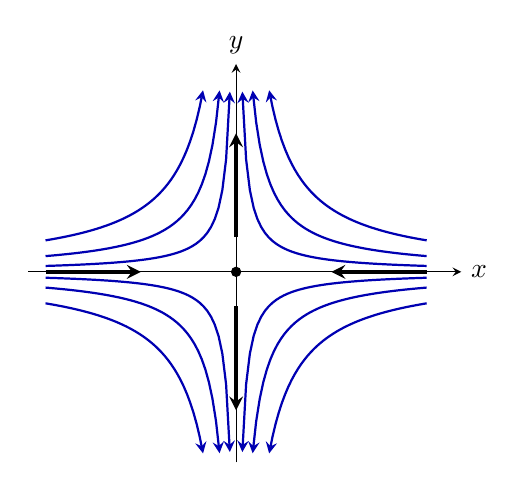
\begin{tikzpicture}[>=stealth, scale=1.1]
    \draw[->] (-2.4,0) -- (2.6,0) node[right] {$x$};
    \draw[->] (0,-2.2) -- (0,2.4) node[above] {$y$};
    \draw[very thick, ->] (2.2,0) -- (1.1,0);
    \draw[very thick, ->] (-2.2,0) -- (-1.1,0);
    \draw[very thick, ->] (0,0.4) -- (0,1.6);
    \draw[very thick, ->] (0,-0.4) -- (0,-1.6);
    \filldraw (0,0) circle (1.5pt);
    \foreach \k in {0.15, 0.4, 0.8} {
        \foreach \sx in {1,-1} { \foreach \sy in {1,-1} {
            \draw[thick, blue!70!black, domain=2.2:\k/2.1, samples=50, ->] plot ({\sx*\x}, {\sy*\k/\x});
        } }
    }
\end{tikzpicture}
\end{center}

\begin{center}
\fcolorbox{orange!85!black}{orange!10}{\parbox{0.92\linewidth}{\centering \textbf{Hasta aquí llegamos en clase (25/11).}\\[0.2em] Quedan el resto de subcasos de autovalores reales y los demás casos de $\sigma(A)$.}}
\end{center}
